\chapter{Project architecture}
\label{ch:architecture}
The described solution is composed of four directories with subprojects (data-gathering, database-manager, data-miner, server), three auto-generating directories with program-related data (logs, flags, data) and a docker-compose.yml file. Each of the four directories has a Dockerfile, and acts as a build context for an image. Additionally, two containers are pulled from the Docker image repository, the MySQL server (\textit{mysql/mysql-server}) and Selenium standalone Firefox webdriver (\textit{selenium/standalone-firefox}).
Figure (\ref{arch:container_dependencies}) shows how the dependencies between containers.

\begin{figure}[h!]
    \centering
    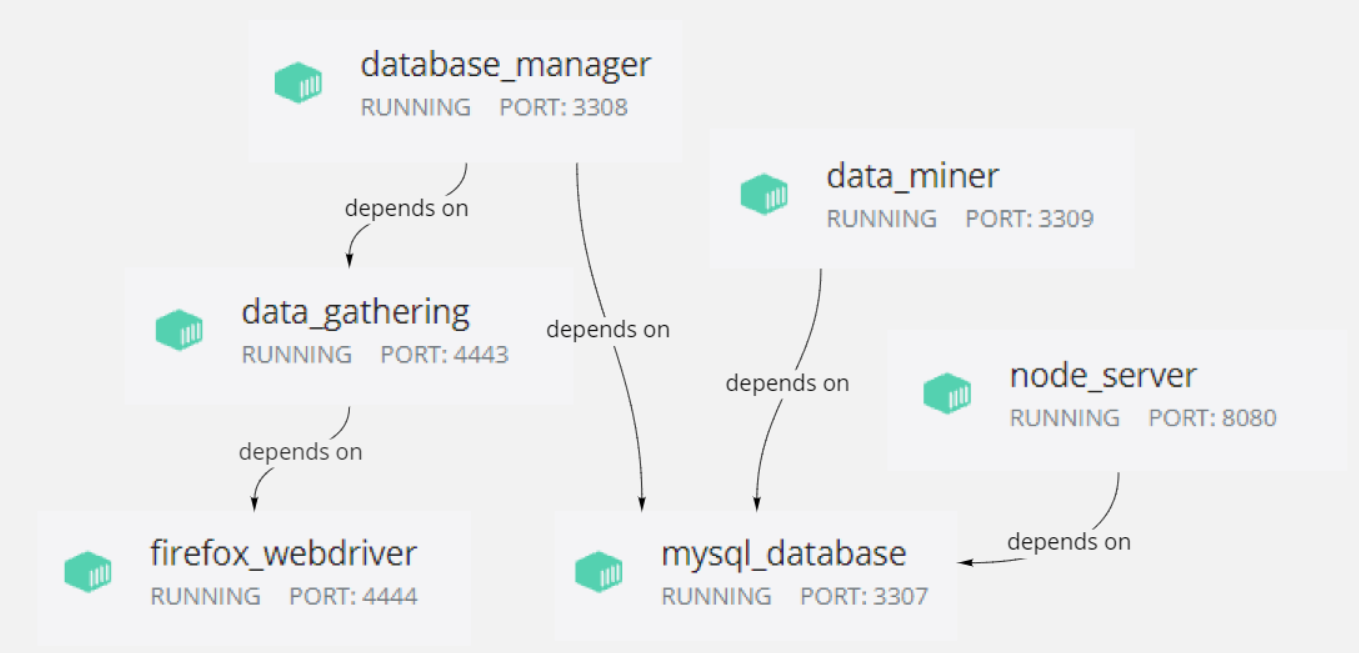
\includegraphics[width=\textwidth]{figures/container_dependencies.png}
    \caption{Boot order of containers (least dependant first)}
    \label{arch:container_dependencies}
\end{figure}

\section{Containers}
The task of the \textit{firefox\_webdriver} container is to provide a constant and reliable access to a browser-like solution for automated page navigation. The \textit{mysql\_database} container hosts a database with persistent memory, storing the major part of the data warehouse and making it accessible to other containers. The \textit{data\_gathering} subsystem automatically collects the web-scraped data in the \textit{data} directory, while \textit{database\_manager} takes this data and passes it to the database. It is important for the \textit{database\_manager} to be slightly delayed with respect to \textit{data\_gathering}, for reasons that are explained in appropriate section of this thesis. The \textit{data\_miner} and \textit{node\_server} containers are dependent only on the database, however here boot order or system state are not as important; these asynchonous containers perform their job properly when the data is ready and don't cause critial failure when it's not, which is enough for the system to run reliably.
Each container has its own virtual storage, so to perform tasks on a shared set of data, either persistence, data binding or both have to be introduced. Additionally, each container exposes one port internally to a port on the host, inside a network encompassing the whole solution.


\section{Services}
The three programs written in Python share similar functions. These are grouped into \textbf{services} by their main utility and by needed external libraries. Each directory contains a \textit{services} module with the following:
\begin{itemize}
\setlength\itemsep{0.3em}
\item \textit{logs\_service} --- responsible for creating a container-specific logs directory with a daily log file and optionally run log file, general logging to file and console. Libraries needed: \textbf{os}, \textbf{time}.
\item \textit{flags\_service} --- this service creates the flags directory, sets up checksum files and provides an interface for everything related to detecting differences in directories or checking the current stage of the data. Libraries needed: \textbf{os}, \textbf{checksumdir}.
\item \textit{data\_service} --- handles everything related to CSV files, translating the scraped data into attributes, loading and saving dataframes, pickling and unpickling the data, all data manipulation pre-mining and ensuring the completeness and correctness of the data. Libraries needed: \textbf{os}, \textbf{sys}, \textbf{shutil}, \textbf{time}, \textbf{pandas}.
\item \textit{web\_service} --- interface for connecting to the webdriver and navigating the pages, finding appropriate elements on the website, implicit and explicit waiting for response, page validation and so on. Libraries needed: \textbf{time}, \textbf{bs4}, \textbf{selenium}.
\item \textit{database\_service} --- manages connection to the database, setting up the tables, updating the schema with new data, as well as creating helper views and additional tables in the data mining part. Libraries needed: \textbf{mysql.connector}.
\end{itemize}

\section{Containers orchestration}
The containers are all started when the \textsc{docker-compose up} command is issued in a root directory of the project. This causes the containers from external images to be loaded first, based on the dependency tree. From there, more control over the mutual cooridation is available via healthchecks or timing. Out of simplicity, the second approach is present in this thesis; i.e. the gathering project is initialized with an immediate 10 seconds delay, so that the webdriver is surely ready before a connection attempt takes place. Similarly, the database managing part is started after 20 seconds, so that the previous container can assess whether there is some new data and any action is needed, or that data can be verified, and marked as ready to be updated to the database. The data mining part is delayed 30 seconds, in case the database is in pre-update state, and other services will start to act on it. However, the most important element of orchestration is shared access to the flags directory, which stores two files with directory checksums, calculated from the ready and complete data after a gathering run. This checksum becomes the new standard and an indicator that the database contents may be outdated.

\section{Data pipeline}
High level overview of the data pipeline (schema).
Where does the data come from? How do I get it?
Where do I validate it? What happens in the directories?
What happens in Docker volumes? What happens in the database?
What is the end result of the pipeline?
What is the speed of consecutive steps?

\begin{figure}[h!]
\centering
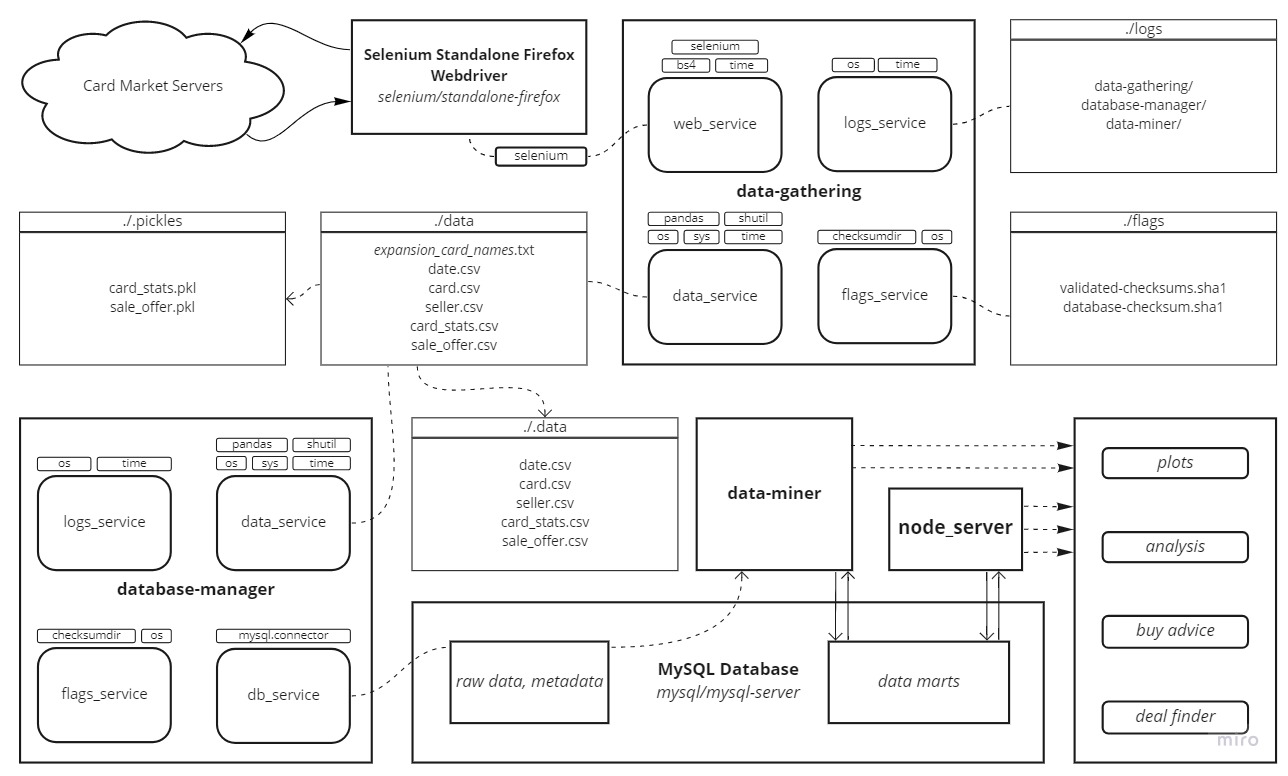
\includegraphics[width=\textwidth]{figures/warehousing.jpg}
\caption{Data pipeline from the server (left-top) to results (right-bottom).}
\end{figure}


\section{Compatilibity}
Is my project compatible with main operating systems?
How does the installation differ on various systems?

